\documentclass[runningheads]{llncs}
\usepackage[T1]{fontenc}

% define lightgray
\usepackage[table]{xcolor}

\usepackage{booktabs}
\usepackage[square,sort,comma,numbers]{natbib}
\usepackage[pdfstartview=XYZ,
bookmarks=true,
colorlinks=true,
linkcolor=blue,
urlcolor=blue,
citecolor=blue,
pdftex,
bookmarks=true,
linktocpage=true, % makes the page number as hyperlink in table of content
hyperindex=true
]{hyperref}

\usepackage{orcidlink} % orcidlink
\usepackage{marvosym} %letter symbol
\usepackage{rotating} % Rotating table
\usepackage{subcaption}
\usepackage{graphicx}
\usepackage{multirow}
\usepackage{amsmath}

%\newcommand{\myvec}[1]{\mathbf{#1}}
\newcommand{\jd}[1]{\scriptsize {\bf \color{red}[JD: #1]}\normalsize}
\newcommand{\mn}[1]{\scriptsize {\bf \color{blue}[MN: #1]}\normalsize}

\title{Generating synthetic data is complicated: Know your data and know your generator}
\titlerunning{Generating synthetic data is complicated}

\author{Jonathan Latner\inst{1 (\text{\Letter})\orcidlink{0000-0002-1825-0097}} \and
Marcel Neunhoeffer\inst{1,2 \orcidlink{0000-0002-9137-5785}}  \and
J\"{o}rg Drechsler\inst{1,2,3 \orcidlink{0009-0009-5790-3394}}}

\authorrunning{Latner et al., \the\year}

%\author[1,2]{Marcel Neunhoeffer}
%\author[1]{Jonathan Latner}
%\author[1, 2, 3]{J\"{o}rg Drechsler}
%\affil[1]{Institute for Employment Research, Nuremberg, Germany}
%\affil[2]{Ludwig-Maximilians-Universit\"at, Munich, Germany}
%\affil[3]{University of Maryland, College Park, USA}

\institute{Institute for Employment Research, Nuremberg, Germany 
\email{\{jonathan.latner, marcel.neunhoeffer,joerg.drechsler\}@iab.de} \and
Ludwig-Maximilians-Universit\"at, Munich, Germany \and
University of Maryland, College Park, USA
}


\begin{document}

\maketitle % typeset the header of the contribution

\begin{abstract} %The abstract should briefly summarize the contents of the paper in 150--250 words.

There is a widely held perception that generating synthetic data is easy.  We show that generating synthetic data is a complicated process that requires one to understand both the original dataset and the synthetic data generator (SDG).  We compare four measures of utility from three SDGs applied to one real-world dataset.  We make two contributions to the literature in this topic area.  First, we show that is just as important to pre-process or clean the data as it is to tune the SDG in order to create synthetic data with high levels of utility. Second, we identify a new type of trade-off.  It has long been understood that there is a trade-off between synthetic data with high levels of statistical utility and high levels of privacy protection, but we show that users who want to create synthetic data must also trade-off different types of statistical utility when comparing the advantages and disadvantages of a given SDG.  

\keywords{Data synthesis \and Data utility \and Microdata}
\end{abstract}



% LENGTH OF SUBMISSIONS.

% Using the above format with 11-point font, the paper should be at most 12 pages excluding the bibliography and appendices, and at most 16 pages total. Committee members are not required to read appendices; the paper should be intelligible without them. Submissions not meeting these guidelines risk rejection without consideration of their merits.

\section{Introduction}
The idea of synthetic microdata\footnote{Throughout the paper, when we refer to data, we are referring to microdata (i.e., one observation per individual unit), as opposed to releases of summary tables.} for statistical disclosure limitation has been introduced more than 30 years ago \cite{rubin1993statistical,little1993statistical,liew1985data} and has gained importance in recent years \cite{drechsler2022challenges,jordon2022synthetic}. The general appeal of synthetic data is obvious: synthetic data promises to mimic the statistical properties of the original data while maintaining the privacy of individual records. In practice, releasing synthetic data means fitting a model to the original data and then generating new data based on this model.  The new interest in synthetic data was spurred by the development of new methods and algorithms to generate synthetic data, many of which are available as open-source software \cite[see, e.g., ][]{nowok2016synthpop,ping2017datasynthesizer,ctgan}. At the same time, private companies offer synthetic data generation to share data while not disclosing any private information as a service for companies and public administration.

This leaves the general impression that generating synthetic data has become easy and that software libraries offer a one-fits-all solution. While it is indeed easy (even for novices) to generate synthetic data, it is hard to generate high-quality data. This paper addresses the question: What makes generating high-quality synthetic data hard? In particular, we focus on the data you want to synthesize and the synthetic data generators (SDG) you wish to use. We show that one must possess good knowledge of the data and the generator when deciding which SDG is appropriate for what data. 

The idea of releasing synthetic data instead of actual data is often understood to have begun in the early 1990s \cite{rubin1993statistical,little1993statistical}.\footnote{We note that several years before Rubin's seminal paper \cite{rubin1993statistical}, an approach was developed for statistical disclosure protection that we might recognize as synthetic data, but they never called it that way \cite{liew1985data}.}  Here, when we refer to data, we are referring to microdata (i.e. one observation per individual unit) as opposed to tabular data (i.e. summary data).  Releasing synthetic data means fitting a model to the original data and then generating new data based on this model so that the released data do not contain information on a real individual unit (person, firm, etc.) that would reveal information that could be used to identify the unit.  The appeal is that the synthetic data mimic the statistical properties of the original data while maintaining the privacy of individual records.

%\mn{marcel.neunhoeffer: The next sentence contradicts the previous sentences. If it is sufficient to release any synthetic data that dosen't contain original records, there is no trade-off.}

While it has long been understood that creating synthetic data are hard because there is a trade-off between creating synthetic data with high levels of statistical utility or high levels of privacy protection, there is now a perception that making synthetic data are easy.  The reason is the availability of open source synthetic data generators (SDGs) and private companies that can generate synthetic data.  In this study, we illustrate why making synthetic data are complicated, but not in a way that is often understood.  Not only is there a trade-off between privacy and utility, there is also a trade-off in types of statistical utility.  While it is possible to design SDGs that perform well on any one utility measure, it is not yet possible to design SDGs that perform well on every utility measure \cite{drechsler2022challenges,jordon2022synthetic}.  As a result, one must possess both knowledge of the data and the generator when deciding which SDG is appropriate for what data.  

\section{Study design}\label{sec:study_design}

In this study, we illustrate the problems in generating high quality synthetic data when there is a disconnect between knowledge of the data and knowledge of the generator.  To do so, we use one dataset, three synthetic data generators (SDGs), and four measures of utility.  The SDGs we use are commonly compared and contrasted in the literature \cite{dankar2021fake,little2022comparing}.  Three utility measures follow Taub et al. \cite{taub2020impact} and Little et al. \cite{little2022comparing}, and are implemented in \textsf{R} from the Synthpop package \cite{nowok2016synthpop} that compare 5 copies of synthetic data to the original data.  The fourth is the duration in time required to create the synthetic dataset \cite{jordon2022synthetic}. Some SDGs that perform well on one or another measure of utility, do not perform well on another. Therefore, users interested in creating synthetic data must trade-off what utility measures are important for their research purpose.

\subsection{Data}

The data we use are called, Social Diagnosis 2011 - Objective and Subjective Quality of Life in Poland (SD2011) and are included as part of the Synthpop package, but are also publicly available.\footnote{ \url{http://www.diagnoza.com/index-en.html}}  There are 35 variables and 5.000 observations, 21 variables are categorical (or factor), and 14 variables are numeric.  

There are two main reasons why we use SD2011 data.  One is data dimensionality, which refers to rows, columns, and unique values within categorical variables.  Data dimensionality affects the duration in time required to generate the synthetic data.  While we do not consider SD2011 to be a high dimensional data set, it is higher dimensional than data used in previous evaluations \cite{dankar2021fake,little2022comparing}.  While previous research used data with more columns, the data contained far fewer rows or if data contained more rows, then they contained fewer columns.  

The second reason is that SD2011 contain many properties of real data, including missing, outlier, or `messy' values, and generated variables.  Previous evaluations used clean data from Census \cite{little2022comparing} or machine learning benchmarks (Kaggle, UCI, OpenML) \cite{dankar2021fake}.  Without denying the value of clean data for evaluation purposes, real data present challenges for SDGs that are not otherwise understood.  For example, some SDGs cannot be used on data with missing values.  Therefore, the ability to synthesize missing values is a stage of development that SDGs must go through before they can be applied to real data.\footnote{Early versions CTGAN could not be used on data with missing values (\url{https://github.com/sdv-dev/CTGAN/issues/39}).}  

\subsection{Synthetic data generators (SDGs)}

{\bf Synthpop} (Version 1.8.0) \cite{nowok2016synthpop} was used. Synthpop is an \textsf{R} package that implements parametric and CART models (classification and regression trees) to generate synthetic data.  CART models are the default.  Synthpop follows a sequential process, where the first variable to be synthesized is generated by random sampling with replacement from the original values, and the subsequent variables are synthesized one at a time, sequentially.  The advantage is one can easily create synthetic data with little tuning.  The disadvantage is that CART, like most tree-based models struggle computationally with categorical variables that contain many values  \cite{little2022comparing}.  

{\bf DataSynthesizer} (Version 0.1.11) was used \cite{ping2017datasynthesizer}.  DataSynthesizer is a Python package that implements the PrivBayes algorithm \cite{zhang2017privbayes}.  PrivBayes is designed to address the challenges associated with a differentially private method for releasing synthetic data outputs from high-dimensional real data inputs.  To achieve this goal, the package implements a Bayesian network model specify the joint distribution of the data.  Joint modeling differs from the sequential approach used by Synthpop.  The advantage is that one can create privacy preserving synthetic data and maintain output scalability with dimensionality.  The disadvantage is that one must sacrifice some amount of utility in continuous variables.   


{\bf CTGAN} (Version 1.9.0) was used \cite{ctgan}.  CTGAN is a Python package that is part of the Synthetic Data Vault package \cite{patki2016synthetic}.  In their original application, GANs were designed to create synthetic images  \cite{goodfellow2014generative}, but the approach was adapted to create synthetic microdata \cite{park2018data}.  GANs simultaneously train two neural networks: a generator and a discriminator. The goal of the generator is to create synthetic data that becomes increasingly indistinguishable from original data.  The goal of the discriminator is to get better at distinguishing between original and synthetic data.  This adversarial process goes back and forth until the discriminator cannot distinguish between the original data and the generated data.  One advantage is that GANs are designed to work well continuous variables, unlike DataSynthesizer.  One disadvantage is that cells in micro data are not informative of neighbors in the same way that pixel cells in a photograph. As a result, GANs can struggle modeling relationships between cells and columns \cite{drechsler202330}.

\section{Know your data}\label{sec:know_your_data}

SD2011 contain a variety of characteristics found in real data that can present a challenge to synthetic data generators (SDGs).  As a result, they must be cleaned prior to applying a SDG.  However, cleaning the data requires knowledge of the data that is not always available to those with knowledge of a given SDG and may not be easy to detect or follow simple rules.  In figure \ref{fig:know_your_data}, we use DataSynthesizer to demonstrate the importance of preprocessing the data, but the point is applicable to all SDGs.

{\bf Missing values.} In real data, it is common for missing values to be coded as either negative values or large positive values (999999).  For example, in the variable \texttt{wkabdur} (Months working abroad in 2007-2011), in original data, 97.5\% of all values are -8.  The interpretation is values of -8 are missing and only 2.5\% of the sample worked abroad between 2007 and 2011.  If these values are not cleaned and coded as missing before applying the SDG, then the SDG will treat these values as correct values to be included in the synthetic data, which will reduce statistical utility.  For example, if we did not code values of -8 as missing in the original data, then values between -8 and 0 would be created in the synthetic data that do not exist in the original data, as shown in figure \ref{subfig:graph_datasynthesizer_wkabdur}.  

{\bf Generated variables.} Generated variables are variables created from the original values.  In SD2011, there are two generated variables.  The variable \texttt{agegr} is generated from \texttt{age} and the variable \texttt{bmi} is generated from the variables \texttt{height}(cm) and \texttt{weight}(kg).  Given that synthesizing any one variable is a challenge, the challenge increases for each additional variable being synthesized, by definition.  It is not necessary to synthesize generated variables and doing so can be problematic.  For example, in the case of \texttt{agegr}, there are 4 missing values in the original data that have non-missing values for age.  This is an error.  However, if we applied the SDG to the original data that included \texttt{agegr}, then it would not only reproduce these missing errors in the synthetic data, but also increase the number of missing values, as shown in figure \ref{subfig:graph_datasynthesizer_agegr}.  Therefore, we recommend dropping generated variables prior to applying the SDG, and then recreate them afterward using synthetic values.  

{\bf Outliers.} For example, in the case of \texttt{bmi}, there is an outlier value of 450, which is the result of \texttt{height} = 149 and \texttt{weight} = NA.  If we calculate weight from bmi and height, then weight equals 999 or one metric ton.  While this value is an error in the original data, what if it were correct and simply an outlier?  If we included the value of 451 in the original data, then values between 451 and 70 would be created in the synthetic data that do not exist in the original data, as shown in figure \ref{subfig:graph_datasynthesizer_bmi}.  Fortunately, in our case, \texttt{bmi} is a generated variable, which we can drop.  However, the existence of outlier values can affect the ability of SDGs to create synthetic data with high levels of utility as well as privacy.  

{\bf Messy values.} In real data, variables include messy values, such as errors or spikes.  An example of an error are the variables for \texttt{smoke} and \texttt{nociga}, where two individuals indicate they do not smoke also indicate they smoke 20 or 22 cigarettes per day, respectively.  An example of spikes is the variable \texttt{nofriend} (number of friends).  In the original data, the variable \texttt{nofriend} appears to be normally distributed below 10, but then clusters at values of 10, 15, 20 and groups of 10 up to the maximum 99.  This is sometimes referred to as `spikey', discontinuous, or semi-continuous values.  As shown in figure \ref{subfig:graph_datasynthesizer_nofriend} and we describe in more detail below, errors and spikes can pose a problem for statistical utility because the models used by SDGs to create synthetic data smooth or attenuate values found in the original data.

\section{Know your generator}\label{sec:know_your_generator}

It can be as important to pre-process or clean the data prior to applying a given SDG as it is to tune a SDG.  To illustrate this, we use three versions of the original data to create synthetic data and compare utility.  SD2011(a) is the raw data.  SD2011(b) codes all negative values that indicate missing values in numeric variables as missing, and all empty values in character variables as missing.  SD2011(c) drops the two generated variables (\texttt{agegr} and \texttt{bmi}) and then recreates them from the synthetic values.  All SDGs were developed with particular data sets or particular problems to solve.  We show what happens if you apply SDGs to real data in order to illustrate that each contain advantages and disadvantages that make the more or less appropriate for any given data set or purpose.  

\subsection{Synthpop} 

We apply Synthpop to SD2011(c) using default values for all hyperparameters.  A feature of CART-based models is that they can produce synthetic data with high levels of statistical utility \cite{little2022comparing,dankar2021fake,drechsler2011empirical}, but they are not computationally efficient with high dimensional data.  While CART-based models are well described elsewhere \cite{breiman2017classification,reiter2005using}, the important point we want to make is that the number and order of categorical variables with a large number of unique values in data sets can affect the duration in time required to synthesize data \cite{raab2017guidelines}.  The result is a trade-off is between statistical utility and computational efficiency in high dimensional data.

To understand how the process of recursive binary splitting used by CART-based models affects the time required to create synthetic data, imagine the following small, simple example.  A data frame with two variables, one continuous (the target) and one categorical variable (the predictor) with three values (a, b, and c).  CART builds a binary tree from the data by splitting the data into subsets that maximize the homogeneity of the target variable.  There are three possible options in the first node: (1 = a; 0 = b,c), (1 = b; 0 = a,c), (1 = c; 0 = ab).  In the second node, 0 can be a dichotomous split.  

The process of splitting categorical variables affects duration time in two ways.  First, the more categories you have, the more options there are to try.  More options require more time, by definition.  Second, the splitting process has to be done each time the variable is used as a predictor.  If a variable with a large number of unique values is ordered early, then the splitting process has to be done for each of the subsequent variables in the model.  

Solutions exist, but limitations remain.  One option is to aggregate categorical variables with a large number of unique values.  The problem is that this can reduce heterogeneity in synthetic data that we would want to preserve.  Another option is to order categorical variables with a large number of unique values at the end, so that they are not used as a predictor as often.  The problem is if there are a sufficient number of variables with a large number of unique values.  For example, if a Census data set contained variables for 3-digit ISO country code, 4-digit ISCO codes (occupation), 4-digit ISIC codes (industry), then it would be difficult to avoid computational problems through ordering.  

To illustrate this, we examine the duration in time required to create synthetic data, i.e. computational efficiency, as shown in table \ref{table:table_sd2011_duration}.  If we load raw SD2011(a) into \textsf{R} as a .csv file as we normally do with a SDG, then Synthpop requires 2,132 seconds (35 minutes and 30 seconds), but we if load SD2011 into \textsf{R} from the Synthpop package, then Synthpop requires 5,474 seconds (91 minutes).  The difference in duration within Synthpop is explained by two variables: \texttt{eduspec} and \texttt{wkabdur}.  Both variables have a large number of unique values (28 and 33, respectively). For some reason, when SD2011 is loaded into \textsf{R} from the Synthpop package, then \texttt{wkabdur} is treated as a character variable, not a numeric variable, as it actually is.  However, if SD2011 is loaded into \textsf{R} from a .csv file, then \texttt{wkabdur} is correctly treated as a numeric variable.  When we treat \texttt{wkabdur} as a numeric variable and place \texttt{eduspec} at the end, then Synthpop requires less than 15 seconds, regardless of how SD2011 is loaded.  Therefore, Synthpop is a computationally efficient SDG with proper preprocessing.

However, the issue reveals a more general problem that Synthpop is sensitive to the number (and order) of categorical variables with large values.  To illustrate this, we added one, two, or three categorical variables with 20, 25, or 30 unique random categorical values to SD2011.  Duration times for Synthpop increase with additional variable and number of unique values.  Therefore, Synthpop is less computationally efficient as the data dimensions increase. 

The trade-off of computational inefficiency is high levels of statistical utility.  We examine parameter estimates and confidence interval overlap (CIO) for two regression models (OLS and LPM), as shown in figure \ref{fig:utility_compare_cio}.  The overlap is higher in the OLS model (ROE = 0.59) compared to the LPM model (ROE = 0.40).  The difference is explained when we examine the parameter estimates.  In the LPM model, Synthpop over estimates the effect of education level on smoking for two values (less than secondary and secondary) as positive and significant.  In the original data, they are positive and insignificant.  The conclusion from synthetic data would be that levels of education affect smoking, but the conclusion from  the original data is that smoking is only related to one level of education (vocational or grammar).  Therefore, even with high levels of CIO, synthetic data from Synthpop is not a substitute for original data.

\subsection{DataSynthesizer}\label{subsec:know_your_generator_datasynthesizer}

A feature of DataSynthesizer is that it implements a Bayesian network model to produce synthetic data.  Like most Bayesian network models, the algorithm implemented by DataSynthesizer assumes that all variables are discrete.  Therefore, DataSynthesizer encodes or discretizes continuous variables into bins and then re-encodes values within a given bin from attribute values in appropriate order from the Bayesian network \cite{ping2017datasynthesizer}.  The result is a trade-off between statistical utility and computational efficiency in high dimensional data.

In DataSynthesizer, there are a number of hyperparameters that can tune, but we focus on two, with all other values set to default.  One hyperparemeter is differential privacy ($\epsilon$-DP). This is a number that quantifies the amount of noise that is introduced into the original data to create synthetic data.  In Datasynthesizer, the default is 0.1 and 0 turns off DP.  We turn off DP for two reasons.  One is to compare to the other synthesizers that do not have a similar hyperparameter.  The second is that in this study, we are not focusing on the well-established trade-off between utility and privacy, but rather the trade-offs within utility measures that receive less attention.

A second hyperparameter are the number of attributes any one variable can have, i.e. parents ($k$).  In a Bayesian Network, there are three possible relationships between X and Y.  Direct dependence where each variable can only have direct attributes (1 parent), weak conditional independence where each variable can have both direct and indirect attributes (2+ parents), and strong conditional independence where all variables are independent (0 parents).  

We begin by applying DataSynthesizer to SD2011(a).  For 0 and 1 parents, pMSE = 0.25; pMSE = 0.2 with 2 parents; and pMSE = 0.21 for 3 parents.  Therefore, 2 parents represents the optimal level of utility.  If we compare pMSE values if k=2 across the three versions of SD2011, then  pMSE = 0.21 for SD2011(a), pMSE = 0.13 for SD2011(b), and pMSE = 0.07 for SD2011(c).  Preprocessing the data can be more important then tuning the synthesizer.  

To illustrate the application of a Bayesian network model to generate synthetic data, we compare frequency counts for the variable \texttt{nofriend} (number of friends), as shown in figure \ref{subfig:graph_datasynthesizer_nofriend}. Below values of 30, DataSynthesizer underestimates high values below 10, and overestimates low values above 20.  Above 30, DataSynthesizer misses the spikes at 30, 40, 50, etc.  The reason is that the Bayesian network discretizes continuous variables into bins and then re-encodes values within a given bin, which fills in values between the spikes that are not representative of the original data.  This reduces statistical utility.

Next, we examine parameter estimates and confidence interval overlap (CIO) for two regression models (OLS and LPM), as shown in figure \ref{fig:utility_compare_cio}.  In both models, overlap is negative, meaning the intervals do not overlap.  Between the two, ROE is better in the LPM model compared to the OLS model (-0.555 and -1.18, respectively), but there is a clear attenuation of the coefficients toward zero in both models.  The interpretation is that estimated coefficients produced by synthetic data from DataSynthesizer are not related to those from original data.

The trade-off of low levels of statistical utility is high computational efficiency, as shown in table \ref{table:table_sd2011_duration}.  For the raw data, DataSynthesizer requires 245 seconds (4 minutes).  At maximum, with three additional variables, each of which contains 30 unique categorical values, DataSynthesizer requires 424 seconds (7 minutes).  Therefore, DataSynthesizer is relatively insensitive to the number and type of variables that are included in the data frame.  However, we note that if a user were to increase the default number of bins, then the resulting increase in levels of statistical utility would come at the cost of a decrease in computational efficiency.

\subsection{CTGAN} 

We apply CTGAN to SD2011(c).  There are two main features of CTGAN that we would like to emphasize.  One, the algorithm assumes that all variables are continuous.  This means that the algorithm transforms categorical variables into continuous variables, where each categorical value occupies its allocated distribution with a Gaussian distribution \cite{patki2016synthetic}.  Two, training and tuning hyperparameters are often central in affecting the quality of the synthetic data output.  

CTGAN contains a number of hyperparameters that one can use to tune the model.  We tune the hyperparameters in three main ways.  First, we maintain a constant number of steps (3.000), but allow the batch size to vary.  Second, we maintain a constant batch size (500), but allow the steps to vary.  Third and finally, we vary the dimensionality of the generator/discriminator networks and the embedding dimension.  In our data, tuning these hyperparameters makes little difference (pMSE $\approx$ 0.16).  Given that, we maintain default values for all hyperparameters with the exception of epochs, which we increase to 600.  One possible explanation for the fact that hyperparameters do not affect the quality of the synthetic data output is that our data are too low dimensional for the parameters to make a difference.  We are aware of other research where tuning hyperparameters does make a difference in the quality of synthetic data output (as yet unpublished).  

Next, we examine parameter estimates and confidence interval overlap (CIO) for two regression models (OLS and LPM), as shown in figure \ref{fig:utility_compare_cio}.  In both models, overlap is negative, meaning the intervals do not overlap.  Between the two, ROE is better in the LPM model compared to the OLS model (-0.420 and -1.48, respectively).  In the OLS model, there is some attenuation toward zero, but in the LPM model the coefficients from synthetic data are upwardly biased.  Either way, coefficients produced by synthetic data from CTGAN are not related to those produced from original data.

The last utility measure is computational efficiency, as shown in table \ref{table:table_sd2011_duration}.  For the raw data, CTGAN requires 331 seconds (5.5 minutes).  At maximum, CTGAN requires 420 seconds (7 minutes).  Therefore, CTGAN is relatively insensitive to the number and type of variables that are included in the data frame.  

Synthetic data from CTGAN does not produce data with high levels of utility, but that does not mean GANs are bad.  CTGAN is not the only GAN in Synthetic Data Vault and multiple other GANs exist.  We note a disconnect in the literature on synthetic data between computer scientists that often rely on GANs without comparing them to CART and statisticians that compare GANs to CART and find that CART models are superior \cite{drechsler202330}.  We are aware of GANs that produce synthetic data with similar utility as Synthpop (as yet unpublished).  It is possible to create a GAN that provides higher levels of utility.  More generally, one must distinguish between the package and the method.  

\section{Conclusion}\label{sec:conclusion}

In contrast to the simplicity of the original idea, and despite decades of progress, the creation of synthetic data include steps that are neither common knowledge nor described in one place.  The conclusion is that making synthetic data is complicated and requires knowledge that may not always exist in one place.  The result is a trade-off is between statistical utility and computational efficiency in high dimensional data.

One must know the data.  Most research examining synthetic data generators (SDGs) uses clean data from Census or Machine Learning libraries.  Unlike clean data, real data contain variables with messy values, which can affect the utility of SDGs.  Despite advertisments to the contrary, it is not possible to simply input real data into a SDG or and high expect high quality synthetic data output.  Our results show that utility of synthetic data is a result of both preprocessing the data and tuning a SDG.  

One must know the generator.  For example, Synthpop produces synthetic data with the high levels of utility, but the CART method that Synthpop uses as the default struggles with computational efficiency with datasets that contain variables with many categories.  It is difficult to imagine applying Synthpop to so-called `big data' with hundreds of variables and millions of observations.  

The other SDGs face different trade-offs.  DataSynthesizer implements a Bayesian network that requires the algorithm to transform continuous variables into categorical variables.  By contrast, CTGAN implements a GAN that requires the algorithm to transform categorical variables into continuous variables.  In both cases, statistical utility is sacrificed for the benefit of computational efficiency.  

Synthetic data is not a substitute for original data \cite{jordon2022synthetic}.  Therefore, prior to making synthetic data, one must decide the purpose.  There is no one size fits all solution and choosing the right SDG is the result of different trade-offs.  



%\subsubsection*{Acknowledgments}
%Use unnumbered third level headings for the acknowledgments. All acknowledgments, including those to funding agencies, go at the end of the paper. Only add this information once your submission is accepted and deanonymized. 

%%%%%%%%%%%%%%%%%%%%%%%%%%%%%%%%
% Tables
%%%%%%%%%%%%%%%%%%%%%%%%%%%%%%%%

\begin{table}
    \centering
    \caption{Duration (in seconds)}
    \rowcolors{1}{white}{lightgray}
    \resizebox{\textwidth}{!}{% latex table generated in R 4.4.0 by xtable 1.8-4 package
% Fri Jul 19 16:14:31 2024
\begin{tabular}{llrrrr}
  \toprule
version & description & ctgan & datasynthesizer & synthpop (csv) & synthpop (package) \\ 
  \midrule
v00 & Raw (SD2011) & 331.01 & 245.37 & 2132.12 & 5474.39 \\ 
  v01 & Without eduspec or wkabdur & 290.30 & 264.43 & 10.99 & 8.45 \\ 
  v02 & Without wkabdur & 337.07 & 351.76 & 13.96 & 11.02 \\ 
  v03 & Without eduspec & 306.46 & 351.24 & 11.39 & 8.92 \\ 
  v04 & Last variables: eduspec-wkabdur & 374.57 & 344.02 & 14.23 & 287.85 \\ 
  v05 & Last variables: wkabdur-eduspec & 419.60 & 339.92 & 14.60 & 3657.55 \\ 
  v06 & as.numeric(wkabdur) and last variable: eduspec & 356.02 & 347.36 & 14.12 & 11.05 \\ 
  v07\_1\_20 & + 1 factor variable (20 values) & 339.05 & 264.96 & 42.23 &  \\ 
  v07\_1\_25 & + 1 factor variable (25 values) & 400.28 & 326.84 & 137.47 &  \\ 
  v07\_1\_30 & + 1 factor variable (30 values) & 339.73 & 269.72 & 363.18 &  \\ 
  v07\_2\_20 & + 2 factor variable (20 values) & 369.74 & 339.45 & 74.96 &  \\ 
  v07\_2\_25 & + 2 factor variable (25 values) & 364.56 & 361.81 & 631.43 &  \\ 
  v07\_2\_30 & + 2 factor variable (30 values) & 373.25 & 346.15 & 1222.54 &  \\ 
  v07\_3\_20 & + 3 factor variable (20 values) & 393.99 & 369.58 & 122.77 &  \\ 
  v07\_3\_25 & + 3 factor variable (25 values) & 401.03 & 383.40 & 881.53 &  \\ 
  v07\_3\_30 & + 3 factor variable (30 values) & 394.44 & 424.64 & 3654.59 &  \\ 
   \bottomrule
\end{tabular}
}
    \label{table:table_sd2011_duration}
    \\
    \raggedright
    \tiny{Notes: Synthpop (csv) indicates that SD2011 was loaded into R from a csv file.  Synthpop (package) indicates that SD2011 was loaded into R from the Synthpop package.}
\end{table}

%%%%%%%%%%%%%%%%%%%%%%%%%%%%%%%%
% Graphs
%%%%%%%%%%%%%%%%%%%%%%%%%%%%%%%%

\begin{figure}[ht]
    \caption{Know your data}
    \label{fig:know_your_data}
    \centering

    \begin{subfigure}{\textwidth}
        \centering        
        \caption{Work abroad duration (in weeks)}
        \resizebox{.9\textwidth}{!}{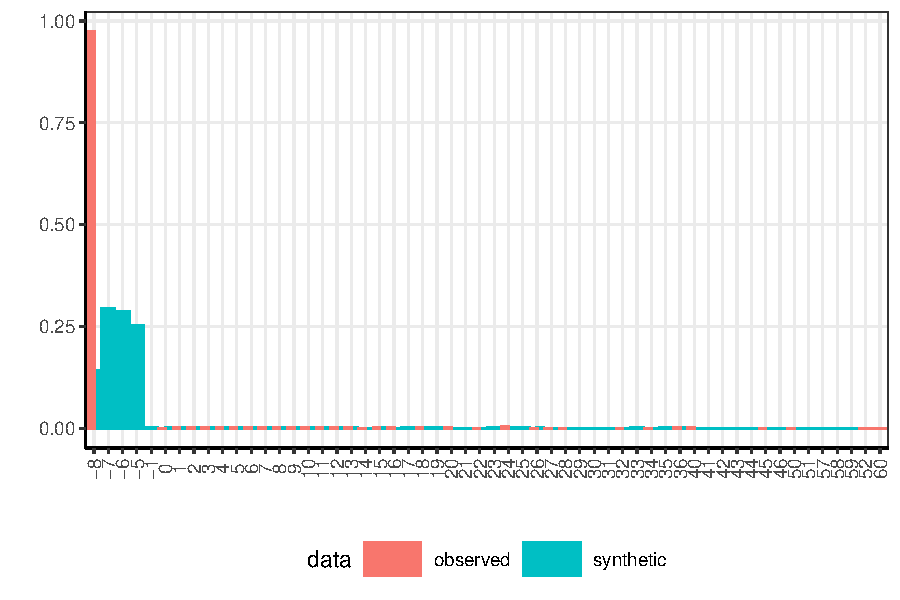
\includegraphics{../graphs/datasynthesizer/datasynthesizer_wkabdur.pdf}}
        \label{subfig:graph_datasynthesizer_wkabdur}
    \end{subfigure}

    \begin{subfigure}{\textwidth}
        \centering        
        \caption{Body mass index (BMI)}
        \resizebox{.9\textwidth}{!}{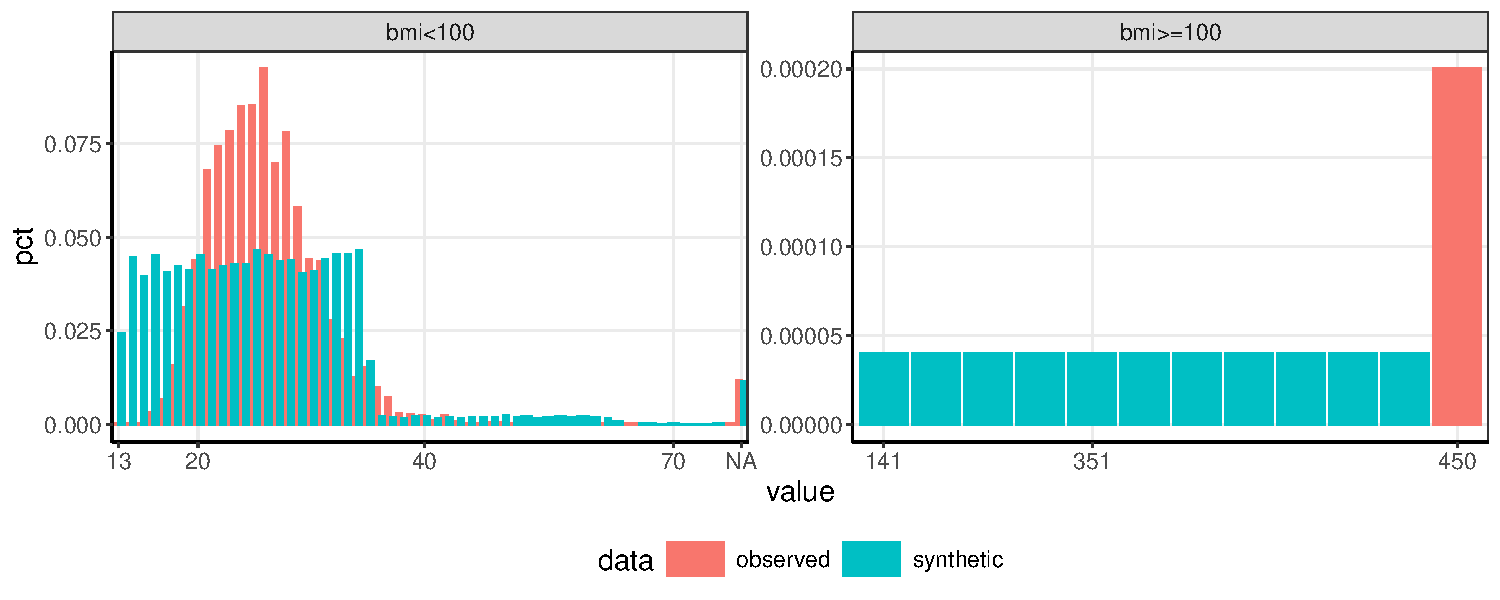
\includegraphics{../graphs/datasynthesizer/datasynthesizer_bmi.pdf}}
        \label{subfig:graph_datasynthesizer_bmi}
    \end{subfigure}

    \begin{subfigure}{\textwidth}
        \centering        
        \caption{Missing values for age group, but non missing values for age}
        \resizebox{.9\textwidth}{!}{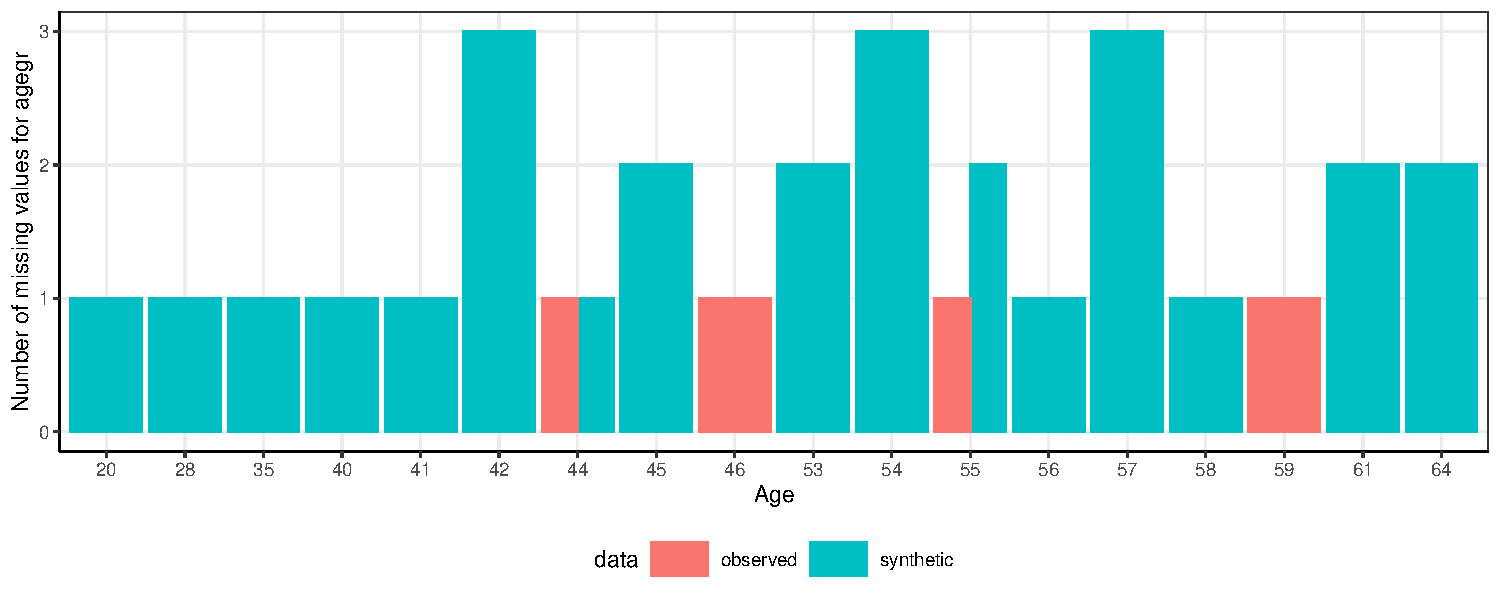
\includegraphics{../graphs/datasynthesizer/datasynthesizer_agegr.pdf}}
        \label{subfig:graph_datasynthesizer_agegr}
    \end{subfigure}

    \begin{subfigure}{\textwidth}
        \centering        
        \caption{Number of friends}
        \resizebox{.9\textwidth}{!}{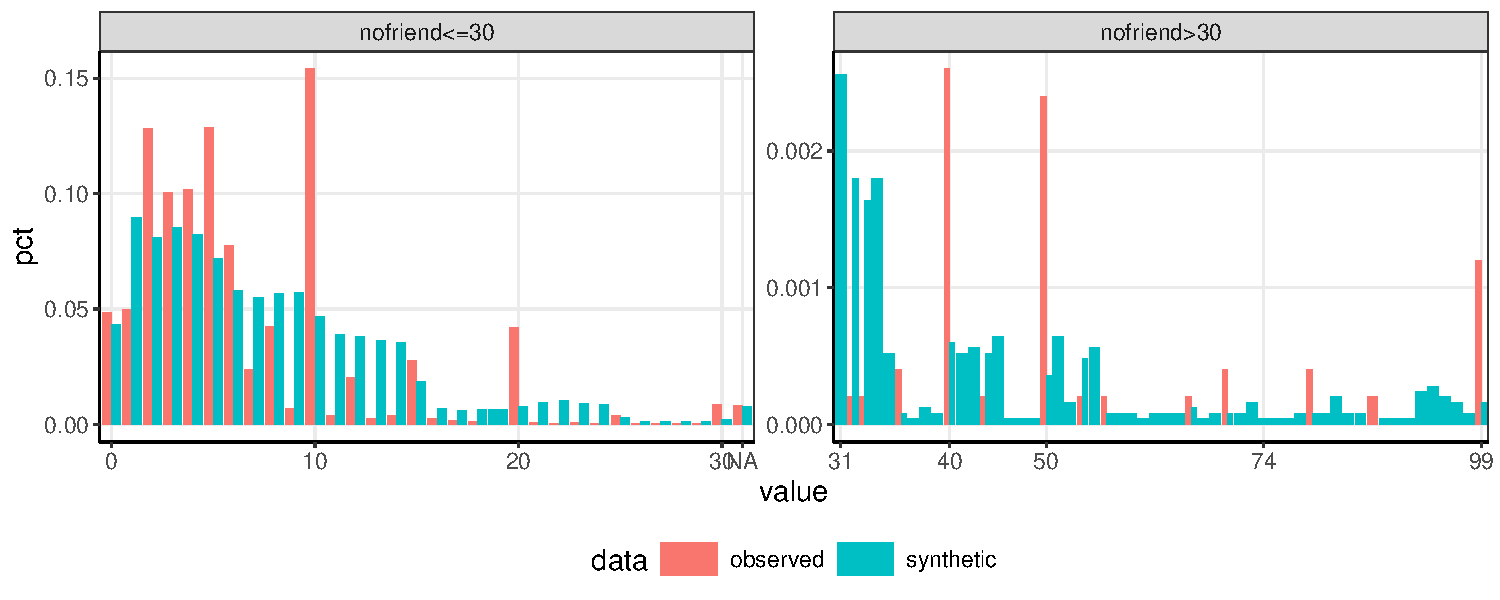
\includegraphics{../graphs/datasynthesizer/datasynthesizer_nofriend.pdf}}
        \label{subfig:graph_datasynthesizer_nofriend}
    \end{subfigure}

\end{figure}

\begin{figure}
    \caption{Confidence interval overlap}
    \resizebox{\textwidth}{!}{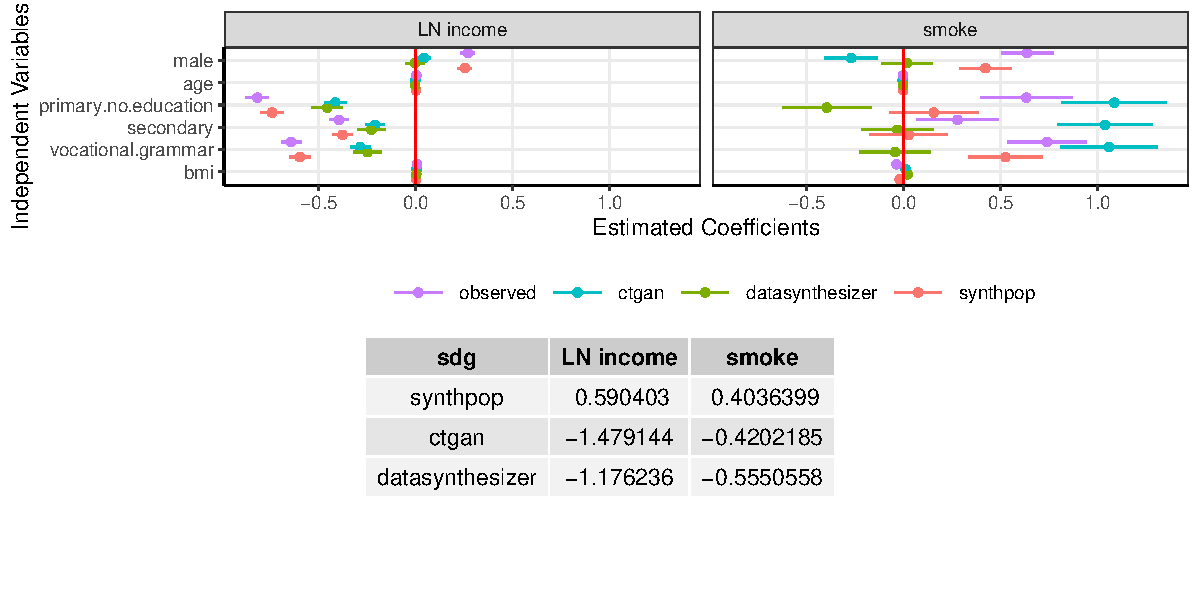
\includegraphics{../graphs/graph_utility_regression_cio_both.pdf}}
    \label{fig:utility_compare_cio}
\end{figure}

%%%%%%%%%%%%%%%%%%%%%%%%%%%%%%%%
% Bibliography
%%%%%%%%%%%%%%%%%%%%%%%%%%%%%%%%
\bibliographystyle{splncs04}
\bibliography{references}

%%%%%%%%%%%%%%%%%%%%%%%%%%%%%%%%
% Appendix
%%%%%%%%%%%%%%%%%%%%%%%%%%%%%%%%

\appendix
\section{Appendix: Utility measures}\label{appendix:utility_measures}
\setcounter{figure}{0}    
\setcounter{table}{0}    

{\bf The propensity score (pMSE)}  is a parametric utility measure that estimates how well one can discriminate between the original and synthetic data based on a classifier \cite{woo2009global,snoke2018general}.  This is sometimes called a `broad'\cite{snoke2018general} or `general'\cite{drechsler2009disclosure} measure of utility or `statistical fidelity' \cite{jordon2022synthetic}.  The main steps are to append or stack the original and the synthetic data, add an indicator (1/0) to distinguish between the two, use logistic regression to estimate the propensity of each record in the combined dataset being `assigned' to the original data, and compare the distributions of the estimated propensity score in the two datasets.  In summary:

%%%%%%%%%%%%%%%%%%%%%%%%%%%%%%%%%%%%%%%%%%
\begin{equation}
pMSE = \frac{1}{N}\sum_{i=1}^{N}[\hat{p}_i - c]^2
\end{equation}
%%%%%%%%%%%%%%%%%%%%%%%%%%%%%%%%%%%%%%%%%%
where $N$ is the number of records in the combined dataset, $\hat{p}_i$ is the estimated propensity score for record $i$, and $c$ is the proportion of data in the merged dataset that is synthetic (0.5). pMSE can be estimated on the complete dataset or subsets of the variables, e.g., all one-way, two-way or three-way combinations. The smaller the pMSE, the higher the analytical validity of the synthetic data.

{\bf Ratio of estimates (ROE)}  is a non-parametric utility measure that compares estimates (frequency or proportion) of values within a variable between the original and synthetic data.\footnote{\url{https://github.com/clairelittle/psd2022-comparing-utility-risk/blob/main/code/ROC_Ratio_of_Counts_Estimates.R}}  The three main steps are (1) create a frequency table (one- or two-way) for the same variable(s) in the synthetic and original data.  (2) Within each table, compare the two estimates for each value by dividing the smaller of these two estimates by the larger one.  (3) Average the resulting within table proportions.  In summary:

%%%%%%%%%%%%%%%%%%%%%%%%%%%%%%%%%%%%%%%%%%
\begin{equation}
    ROE = \frac{1}{N} \sum^{N}_{i=1} \left( \frac{\text{min}(y_{orig}^i,y_{synth}^i)}{\text{max}(y_{orig}^i,y_{synth}^i)} \right)
\end{equation}
%%%%%%%%%%%%%%%%%%%%%%%%%%%%%%%%%%%%%%%%%%
where $N$ is the number of values within a table, $y^i_{orig}$ is the estimate from the original data and $y^i_{synth}$ is the corresponding estimate from the synthetic data.  The higher the ROE, the higher the analytical validity of the synthetic data.  

Here, we examine three variables, a continuous variable, \texttt{bmi} (Body mass index), a categorical variable, \texttt{edu} (Education), and a third variable \texttt{nofriend} (number of friends), which is a continuous variable that contains `spikey' values.  

{\bf The confidence interval overlap (CIO)} is a parametric utility measure that compares 95\% confidence intervals between the same regression model applied to synthetic and original data \cite{karr2006framework}.  This is sometimes called a `specific'\cite{snoke2018general} or `narrow'\cite{drechsler2009disclosure} measure of utility.  The main steps are to average the difference between the upper and lower bound estimates of the confidence interval for each independent variable in the model.\footnote{\url{https://github.com/clairelittle/psd2022-comparing-utility-risk/blob/main/code/CIO_Confidence_Interval_Overlap.R}} In summary:

%%%%%%%%%%%%%%%%%%%%%%%%%%%%%%%%%%%%%%%%%%
\begin{equation}
    CIO = \frac{1}{N} \sum^{N}_{i=1} \frac{1}{2}\left(\frac{\text{min}(u_o,u_s) - \text{max}(l_o,l_s)}{u_o-l_o} + \frac{\text{min}(u_o,u_s) - \text{max}(l_o,l_s)}{u_s-l_s}\right)
\end{equation}
%%%%%%%%%%%%%%%%%%%%%%%%%%%%%%%%%%%%%%%%%%
where $N$ is the number of independent variables, and $u_o,l_o$ and $u_s,l_s$ are the respective upper and lower bounds of the confidence intervals for the original and synthetic data.   The higher the CIO, the higher the analytical validity.  

Here, we estimate two regression models, an OLS model with a continuous dependent variable (\texttt{LN Income}) and a LPM model with a dichotomous dependent variable (\texttt{smoke}).  In both models, the independent variables are \texttt{gender}, \texttt{age}, \texttt{education}, and \texttt{bmi}.  


{\bf Computational efficiency} is the duration in time (in seconds) required to create one single synthetic dataset from a given SDG.\footnote{In terms of computing power, SDGs were run on a 2022 Macbook Air with 16GB of RAM and an M2 Chip with 8‑Core CPU, 8‑Core GPU, and a 16‑Core Neural Engine.  All SDGs were run one at a time in order to minimize computational power problems from parallelization.}  This is sometimes referred to as `efficiency'\cite{jordon2022synthetic} or `output scalability' \cite{zhang2017privbayes}.  The basic idea is that the algorithms used by SDGs can suffer from the curse of dimensionality.  

\end{document}
